%!TeX root = thesis-main.tex
\chapter{Cyber-Physical Swarms}\label{chap:cpsw}\mtcaddchapter
\minitoc% Creating an actual minitoc
The aim of this section is to elucidate the concept of \textit{Cyber-Physical Swarms}, 
 distinguish systems that align with our conceptual framework (an overview is given in \Cref{fig:overview-cpsw}), 
 and identify research domains grappling with analogous challenges. 
% 
\begin{figure}
    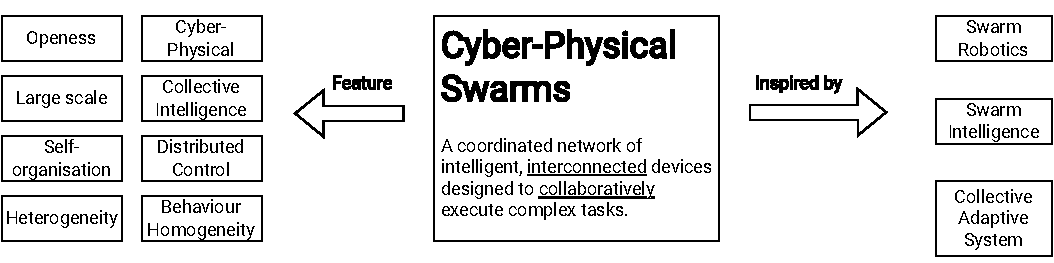
\includegraphics[width=\textwidth]{chapters/img/cyber-physical-swarms-overview.drawio.pdf}
    \caption{Overview of \acf{cpsw} and its related concepts}\label{fig:overview-cpsw}
\end{figure}
\section{Overview}
The term refers to a network of computational nodes working in concert to address collective problems, 
 akin to naturally occurring swarm phenomenam---in the following will be also reffered as ``swarm'' system or ``swarm-like'' systems.
%
The architecture of these systems comprises a large array of interconnected nodes, 
 numbering in the hundreds or thousands. 
% 
Importantly, these networks are \textit{open}, 
 implying that the total node count is not predetermined. 
% 
As a result, 
 the emergent collective behaviour should exhibit \textit{scale-independence}, 
 ensuring that the same programmatic logic applies across small and expansive networks alike.
%
In these systems, each node is tethered to a \textit{physical} entity through sensors and can influence its environment via actuators. 
 This integration of computational and physical elements justifies the term ``cyber-physical''. 
 The nodes may exhibit heterogeneity in hardware or other attributes, 
 yet they maintain a \emph{homogeneous} local behaviour, executing identical local algorithms.
%
Nodes operate with a focus on collective goals, 
 as opposed to individualistic or selfish objectives, 
 thereby adhering to a collaborative ethos.
%
However, each node can still have local objectives, 
 which are not necessarily aligned with the global ones.
% 
Given that centralization is not feasible, 
 the architecture relies on distributed control mechanisms. 
 While modern computing paradigms such as cloud or edge infrastructures are applicable, 
 it is imperative that the system be capable of swift local responses. 
 This is especially critical given that these are often \emph{critical systems}, 
 where delays in decision-making could have severe repercussions.

In concluding, 
 it is pertinent to clarify that the focus of this study is on the \textit{macro-level} behaviours of the swarm, 
 rather than the \textit{micro-level} interactions. 
 Rather than characterizing the collective through emergent properties, 
 the intention is to define a \emph{globally} desirable structure.

%As for related concepts, 
% \acp{cpsw} can be considered a subset of Complex Adaptive Systems~\cite{holland1992complex}. 
% However, our framework imposes additional conditions not universally found in standard definitions of complex systems, 
% such as many collaborative agents.
% 
%Collective Adaptive Systems~\cite{DBLP:journals/corr/abs-1108-5643} closely resemble our definition of \acp{cpsw}, 
% but they diverge in that agents in our framework are geared toward \emph{collective} goals 
% and exhibit homogeneous behaviour.

In the subsequent section, 
 the concept of \acp{cpsw} will be elucidated through a range of examples. 
 These will encompass both existing and prospective applications to provide a comprehensive understanding of the field.
\section{Vision examples}\label{chap:cpsw:vision}
\subsection{Wild-fire monitoring in extensive forests}
Canada is renowned for its lush forests, 
 which cover approximately one-third of the nation's landmass, 
 making it one of the countries with the largest forested areas globally. 
These green expanses are not only a source of natural beauty but also play a crucial role in maintaining ecological balance. 
 However, the increasing impact of climate change has led to a surge in wildfires, 
 causing widespread devastation to both local flora and fauna.
 Consider for instance the 2023 wildfires, 
 which burned over 43 million acres, 
 that is about 5\% of the entire forest area of Canada~\cite{enwiki:1178342069}. 

To address this pressing issue, 
 there is a growing consensus on the need for proactive and localized interventions. 
 Specialized monitoring systems are essential for keeping tabs on vulnerable regions, 
 especially given the impracticality of relying solely on human observation due to the vastness of these areas. 
 One innovative solution might be the deployment of a sophisticated network of environmental sensors, strategically placed to monitor temperature, humidity, and other fire-prone conditions. 
 These sensors might be complemented by a swarm of drones equipped with advanced imaging and data collection capabilities.

The system operates through ongoing collaboration between ground-based sensors and aerial drones. 
 The drones provide a bird's-eye view of the landscape, 
 allowing for real-time monitoring of a wide array of nodes across large geographical expanses. 
 This integrated approach enables the early detection of potential fire hazards, 
 thereby facilitating the pre-emptive mobilization of emergency services.

However, the implementation of such a comprehensive monitoring system comes with its own set of challenges. 
 Each sensor or drone has a limited operational range and can only provide a \emph{partial} view of the overall system. 
 Therefore, robust data fusion algorithms are necessary to merge information from multiple sources into a cohesive and actionable overview. 
 Environmental conditions are also highly dynamic, requiring the system to \emph{adapt} in real-time to changing variables such as wind speed, temperature fluctuations, and precipitation levels.

In specific regions where the risk is elevated
 ---such as areas with active fires or reduced visibility due to smoke or fog---there may be a need for deploying additional sensors and drones. 
 Given that drones have limited battery life and need to be recharged, 
 the system must be capable of \emph{self-organizing} to ensure uninterrupted monitoring. 
 This is particularly challenging considering that the number of deployed devices could easily exceed thousands of units across the extensive area of interest.

Moreover, the system must be highly responsive to emergency conditions. 
 This necessitates that each device, whether a sensor or a drone, 
 should be equipped with \emph{edge computing} capabilities for performing local analyses. 
 These local analyses can then be used to trigger collective alarms, 
 ensuring immediate action is taken to mitigate the risk of wildfires.
\subsection{Crowd steering}
Concert venues (or public event like a soccer match) 
 are often filled with an energetic and enthusiastic crowd, 
 eager to enjoy live performances. 
 These events can attract tens of thousands of attendees, 
 making crowd management a critical concern for both safety and enjoyment. 
% 
However, traditional methods of crowd control, 
 such as barriers and security personnel, 
 are increasingly proving to be inadequate in the face of evolving challenges like sudden surges or emergency situations. 
 Take, for example, the 2019 stampede at the San Carlo place in Turin, 
 where a sudden downpour led to chaotic movements among the crowd, 
 resulting in thousands minor injuries and three deaths~\cite{enwiki:1164182872}.

To address this complex issue, 
 there is a growing interest in leveraging technology for more effective crowd steering. 
 One promising approach might be to equip each attendee with \emph{smart} bracelets or utilize their smartphones, 
 both of which have computational capabilities. 
 These devices can communicate only with each other, 
 forming a dynamic and adaptive network.

The system functions through real-time data exchange 
 between the individual devices %and strategically placed sensors around the venue. 
 The individual smart devices provide a ``ground-level'' perspective, 
 allowing for a granular understanding of crowd behaviour.

This collaborative approach enables the system to identify potential issues before they escalate. 
 For instance, if a particular section of the venue becomes too crowded, 
 the system can send alerts or directions to the smart devices in that area, 
 advising attendees to move to less crowded sections. 
 This facilitates the proactive redistribution of the crowd, 
 thereby averting potential safety hazards.

However, implementing this advanced crowd steering system is not without challenges. 
 Each smart device only has a \emph{limited} computational capacity 
 and can provide just a \emph{partial} view of the overall crowd dynamics. 
Therefore, sophisticated algorithms are needed to aggregate 
 this fragmented data into a comprehensive and actionable overview. 
 Additionally, the system must be able to \emph{adapt} rapidly to changing conditions, 
 such as sudden weather changes or unexpected incidents during the concert.

In specific situations where immediate action is required 
 -- such as medical emergencies or security threats -- 
 there may be a need to send targeted alerts or instructions to specific groups of attendees. 
 Given that smart devices have limited battery life, 
 the system must also \emph{self-organize} to prioritize critical alerts and instructions, 
 ensuring that the crowd management remains effective throughout the event.

Moreover, the system must be highly responsive to real-time conditions. 
 This necessitates that each smart device should compute locally, 
 allowing for point-wise decision-making. 
 These local analyses can then trigger \emph{collective} actions, 
 such as coordinated movements or emergency evacuations, 
 ensuring that immediate and effective measures are taken to maintain crowd safety.

\subsection{Autonomous vehicles}
In a not-so-distant future
 where human-driven cars have become a thing of the past, 
 cities will be bustling with \emph{swarms} of autonomous vehicles. 
% 
These self-driving cars will revolutionize urban transportation, 
 offering a safer and more efficient means of getting from one place to another. 
Indeed, considering the current situation, 
 where the number of accidents and traffic jams is increasing (only in 2023, there were over 5 million accidents worldwide\footnote{\url{https://www.forbes.com/advisor/legal/car-accident-statistics/}}), 
 this is a very appealing scenario.
% TODO here put some statistic abou accidents and traffic jams  
However, the complexity of managing these autonomous fleets is far from trivial, 
 especially during peak hours or special events. 
%
Take for example Tokyo,
 where on average it is estimated that
 over 1 million of cars enter to the metropolitan area every day\footnote{\url{https://www.statista.com/statistics/1191368/shutoko-average-daily-traffic-volume/}}.

To tackle this intricate challenge, 
 there is a growing emphasis on the need for advanced management systems capable 
 of steering these autonomous vehicles effectively. 
 Each vehicle will be equipped with powerful onboard computers 
 and an array of sensors, 
 enabling them to communicate not only with a centralized traffic management system 
 but also with each other.

The system will operate through continuous data 
 exchange between individual cars 
 and strategically located infrastructure sensors. 
 These sensors monitor various parameters such as traffic flow, 
 road conditions, and even weather. 
 Autonomous cars provide a ``street-level'' perspective, 
 allowing for real-time adjustments to routing algorithms 
 and speed controls.

This collaborative approach enables the system to pre-empt potential bottlenecks and accidents. 
 For instance, if a major sporting event ends, 
 causing a sudden influx of ride requests, 
 the system can dynamically reroute cars to manage the increased demand efficiently. 
 This proactive approach minimizes congestion and enhances overall traffic flow.

However, the deployment of such a sophisticated system is fraught with challenges. 
 Each autonomous car has a \emph{limited} sensor range and can only offer a \emph{partial} view of the overall traffic landscape. 
 Therefore, advanced machine learning algorithms are essential to integrate this fragmented data into a cohesive and actionable real-time model. 
 Additionally, the system must be capable of \emph{adapting} quickly to changing conditions, such as road closures, accidents, or even fluctuating demand patterns.

In specific scenarios where immediate action is required
 ---like emergency vehicle passage or sudden road closures---
 there may be a need to prioritize certain routes or vehicles. 
 Given that each car operates on a finite energy source, the system must \emph{self-organize} to ensure that cars with lower battery levels are routed to charging stations without disrupting the overall traffic flow.

\section{Characteristics}
Drawing from the overview and the diverse examples provided, 
 several distinct characteristics emerge that set \acp{cpsw} apart from other large-scale 
 distributed systems. 
% 
These unique traits not only define the essence of \acp{cpsw} but also pose specific challenges in their design and implementation. 
 Each of these characteristics will be discussed in detail below.

\paragraph*{Scale}
\acp{cpsw} are inherently scalable, 
 often comprising hundreds or even thousands of interconnected nodes. 
 The behaviour scale independence ensures that the same programmatic logic can be applied across networks of varying sizes, 
 making them highly adaptable to different application scenarios.
 In doing this, is essential to capture the right collective abstraction that 
 allows both to help the developers to think in terms of the collective behaviour
 and to effectively design the collective behaviour itself.

\paragraph*{Device Heterogeneity}
While the nodes in a \ac{cpsw} may possess varying hardware capabilities and attributes, they are engineered to operate cohesively. Interoperability stands as a fundamental requirement for these systems, particularly because they often incorporate a diverse array of devices manufactured by different vendors. In today's Internet of Things (IoT) landscape, semantic interoperability presents a significant challenge. Devices from various vendors might employ divergent communication protocols or data formats, complicating the task of achieving seamless interaction. This heterogeneity isn't limited to communication protocols; it also extends to computational power, sensor types, and other attributes. Such diversity introduces an additional layer of complexity in system design, necessitating the identification of a common framework that enables effective communication and collaboration among the devices.
\paragraph*{Behaviour Homogeneity}
Despite the diverse hardware configurations, 
 nodes within a \ac{cpsw} display consistent behaviour at the local level.
 They run the same local \emph{algorithms}, thereby achieving the system's collective objectives in a standardized way. 
 However, it is important to clarify that ``homogeneous behaviour'' does not imply that all nodes do the same thing at the same time.
 Indeed, given the system's inherently distributed and potentially expansive nature, 
 the input received by one node may differ from that of another, 
 leading to variations in local behaviour.

\paragraph*{Distributed Control}
Centralized control mechanisms are often impractical in \acp{cpsw} due to their scale and complexity. 
 As a result, these systems rely on distributed control algorithms that enable nodes to make local decisions that collectively contribute to global objectives.

\paragraph*{Self-organization}
One feature of \acp{cpsw} is their ability to self-organize. 
Nodes can dynamically adapt to changing conditions, reconfiguring themselves to maintain system integrity and performance. 
This is particularly important in scenarios where the environment is unpredictable or hostile.

\paragraph*{Openness}
\acp{cpsw} are typically open systems, meaning that the total node count is not predetermined. 
New nodes can join or leave the network dynamically, requiring the system to be flexible enough to accommodate these changes without compromising its functionality.

\paragraph*{Collective Intelligence}
The nodes in a \ac{cpsw} work collaboratively to achieve common goals, displaying a form of collective intelligence. 
This is facilitated by advanced algorithms that enable the system to learn from its environment and adapt its behaviour accordingly.

\paragraph*{Cyber-physical Interactions}
The term ``cyber-physical'' aptly describes the integration of computational and physical elements in \acp{cpsw}. 
 Each node is usually connected to a physical entity via sensors and can influence its environment through actuators. 
 This seamless integration is crucial for applications that require real-time interaction with the physical world.

\section{Related concepts}
\begin{table}[h]
    \centering
    \resizebox{\textwidth}{!}{%
    \begin{tabular}{|c|c|c|c|c|}
    \hline
                                & MAS                         & Swarm Robotics          & CAS          & \ac{cpsw}         \\ \hline
    Scale                       & Dozens                      & Hundreds                & Thousands    & Thousands    \\ \hline
    Capabilities                & Heterogenous                & Homogenous              & Heterogenous & Heterogenous \\ \hline
    Behaviours                  & Heterogenous                & Homogenous              & Heterogenous & Homogenous   \\ \hline
    Control                     & Centralized/Distributed     & Centralized/Distributed & Distributed  & Distributed  \\ \hline
    Cyber-Physical              & Yes/No    & Yes & Yes/No  & Yes  \\ \hline
    \end{tabular}%
    }
    \caption{Summarized comparison between MAS, Swarm Robotics, CAS and \ac{cpsw}}
    \label{table:your_label}
\end{table}
This section will discuss some of the related concepts that are closely aligned with \acp{cpsw} summarized in \Cref{fig:overview-cpsw-taxonomy}.
\begin{figure}
    \centering
    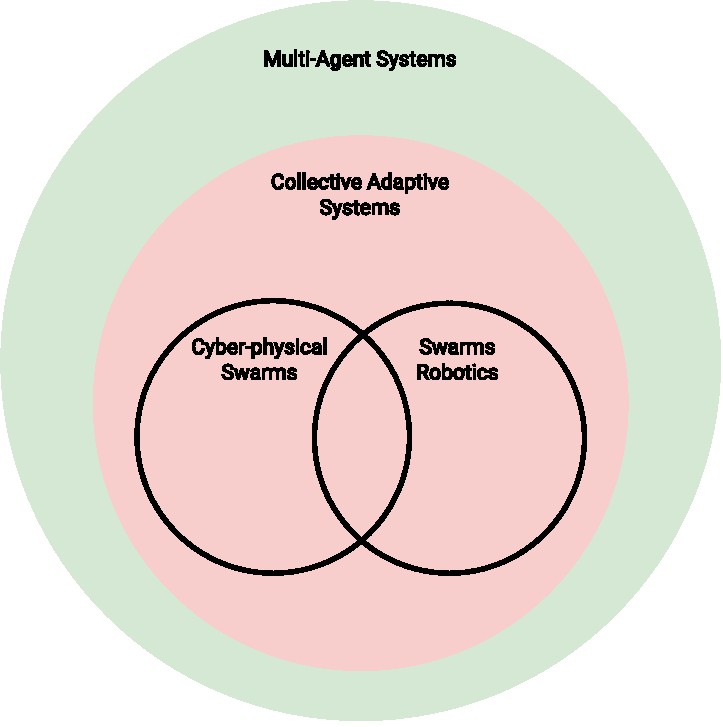
\includegraphics[width=0.6\textwidth]{chapters/img/cyber-physical-swarms-taxonomy.drawio.pdf}
    \caption{Taxonomy of \acf{cpsw} w.r.t related Systems}\label{fig:overview-cpsw-taxonomy}
\end{figure}
%% TODO: add more context of MAS system? gerarchy, organisation, etc.
\paragraph*{Multi-Agent Systems}
In the realm of computational systems, a \ac{cpsw} can be closely related to a Multi-Agent System (MAS), 
 with a specific emphasis on being a \emph{many}-agent system. 
 In a MAS, multiple autonomous agents interact with each other to achieve specific objectives. 
 These agents are capable of sensing their environment, making decisions based on their observations, and then acting upon those decisions. 
 The key difference in a \ac{cpsw} is the scale and the integration of physical components, such as sensors and actuators, which allows for real-time interaction with the environment.

In a \ac{cpsw}, agents are not just virtual entities but are tethered to physical components, making them cyber-physical agents. 
 These agents continuously engage in a cycle of \emph{repeated} sensing, computation, communication, and actuation to achieve collective behaviours. 

One of the significant challenges in designing a \ac{cpsw} is the high stochastic of the environment. 
 Unlike controlled settings where outcomes can be predicted with a high degree of accuracy, \acp{cpsw} often operate in dynamic and unpredictable environments. 
 This makes it nearly impossible to pre-program optimal behaviours for all agents. 
 The agents must, therefore, be capable of adapting their behaviours in real-time based on their sensory inputs and the inputs from other agents in the network. 
 This requires sophisticated algorithms that can handle uncertainty and make near-optimal decisions in real-time.

Moreover, the agents in a \ac{cpsw} are designed to work collaboratively to achieve collective goals, 
 rather than pursuing individual objectives. 
 This is in contrast to some MAS where agents might have conflicting goals. 
 In a \ac{cpsw}, the focus is on achieving a form of collective intelligence through distributed computing and decision-making. 
 Agents share information and coordinate their actions to solve complex problems that are beyond the capabilities of any single agent.

In summary, while \acp{cpsw} share similarities with MAS in terms of multi-agent interaction and decision-making, they extend the concept by incorporating large-scale, cyber-physical integration, and a focus on collective intelligence. 
 The challenges in designing \acp{cpsw} are manifold, ranging from handling the stochastic nature of the environment to ensuring robust and adaptive collective behaviours.

\paragraph*{Swarm intelligence} It is an interdisciplinary field that draws inspiration from the collective behaviours observed in social animals, 
 such as ants, birds, and fish, to develop computational algorithms and systems. 
 Initially, the focus was primarily on Swarm Robotics, 
 where the objective was to create robotic systems that could emulate the complex behaviours seen in natural swarms. 
 The methodology employed is fundamentally bottom-up. 
 Designers and researchers study the behaviours of individual animals in their natural habitats to understand the rules or heuristics they follow. 
 These individual behaviours are then modelled computationally to observe how they contribute to the emergence of collective intelligence in a swarm. 
 One seminal concept that emerged from this line of inquiry is \textit{stigmergy}~\cite{DBLP:journals/fgcs/DorigoBT00}. 
 Stigmergy is a form of indirect communication and coordination where agents in a swarm interact with each other by modifying a shared environment, rather than through direct communication.

In recent years, the focus of swarm intelligence has evolved to concentrate more on algorithmic aspects. 
 Researchers have started to leverage the principles of collective behaviour to develop optimization algorithms that can solve complex computational problems. 
 These algorithms are particularly useful in scenarios where traditional optimization methods are computationally expensive or fail to find optimal solutions within a reasonable time frame. 
 Some of the most well-known algorithms that have emerged from Swarm Intelligence research include Ant Colony Optimization (ACO)~\cite{DBLP:journals/tsmc/DorigoMC96}, Particle Swarm Optimization (PSO)~\cite{DBLP:conf/icnn/KennedyE95}, and Flock of Starling Optimization (FSO)~\cite{DBLP:series/sci/FulgineiS11}. 
Each of these algorithms has its own set of rules and heuristics, modelled after the specific animal behaviours they are inspired by, and they have been applied successfully in various domains such as network design, resource allocation, and data clustering.

While these optimization algorithms offer valuable methodologies and have broad applicability, they are not the central focus of this thesis. 
 Differently, the focus is in harnessing the \emph{principles} of Swarm Intelligence to develop \emph{artificial} systems that can achieve similar collective behaviours through mechanisms of \emph{self-organization}. 
 Unlike traditional Swarm Intelligence algorithms that often aim to \textit{mimic} nature, this thesis draw \textit{inspiration} from natural systems to understand the fundamental principles that make these systems \emph{robust}, \emph{scalable}, and \emph{adaptable}. 
 The ultimate goal is to exploit these principles to design and implement artificial swarm systems that can operate effectively and efficiently in complex, dynamic, and potentially hostile environments. 
 
\paragraph*{Swarm robotics}

Historically, 
 the field of swarm robotics has its roots in the early approaches to swarm intelligence. 
 Over time, it has evolved to become the \textit{engineering} arm of swarm intelligence, 
 focusing on the \emph{practical} aspects of building and maintaining swarm systems. 
 The overarching goal of \emph{swarm engineering} is to establish a rigorous methodology for the entire lifecycle of a swarm robotics system, 
 from conceptualization to operation and maintenance~\cite{DBLP:journals/swarm/BrambillaFBD13}.

In traditional Swarm Robotics, the primary focus is on \textit{robots} that are \emph{autonomous}, \emph{situated}, and operate under \emph{no central control}. 
 These robots are designed to interact with each other and their environment to achieve collective goals. 
 \ac{cpsw} extends this paradigm to include other ``swarm-like'' systems that may not necessarily involve robots. 
 Examples include crowds of people in public spaces, 
 large-scale IoT networks, and smart city infrastructures. 
 These systems share many similarities with swarm robotics, 
 such as the need for autonomy, 
 localized decision-making, 
 and collective behaviour, but they also present unique challenges and opportunities.

One of the most promising avenues for extending the principles of swarm robotics to these other domains is the emerging field of \textit{automatic design}~\cite{DBLP:journals/firai/FrancescaB16}. 
 In automatic design approaches, 
 the control logic for the agents in the swarm is not manually programmed but is instead derived through optimization techniques such as \textit{genetic algorithms} or \textit{Multi-agent Reinforcement Learning}.
These methods aim to optimize a \textit{global} utility function that captures the overall objectives of the swarm. 
 This is particularly appealing for \acp{cpsw}, 
 where the complexity and scale of the system make manual programming impractical.

In summary, 
 the principles and methodologies developed in swarm robotics provide a strong foundation for the engineering of \acp{cpsw}. 
 However, the unique challenges and complexities of \acp{cpsw} require further innovation. 
 By leveraging the principles of swarm intelligence,
 we can create more robust, adaptable, and intelligent \acp{cpsw} that can operate effectively in a wide range of applications and environments.

\paragraph*{Collective Adaptive Systems}
Collective adaptive systems are a broad class of systems composed of agents 
 (potentially heterogeneous) capable of adapting to environmental conditions 
 while striving to achieve a collective goal through the emergence of individual node cooperation. 
%
Typically, individual units are simple and draw strong inspiration from natural systems. 
 In these systems, which are adaptive by nature, 
 there is interest in incorporating \emph{self-*} properties (in fact, these CAS are sometimes discussed as collective self-adaptive systems). 
%
These properties include \emph{self-healing}, \emph{self-optimization}, and \emph{self-configuration}. 
Self-healing refers to the system's ability to recover from failures without human intervention. 
Self-optimization means the system can improve its performance over time based on feedback. Self-configuration allows the system to adapt to changing conditions without requiring manual adjustments. 
These self-* properties contribute to the system's overall \emph{resilience} and \emph{efficiency}.

\ac{cpsw} can be understood as a specialized subset of the broader CAS.
This specialization arises from two key distinguishing characteristics:
i) The involved entities are not merely digital but also have a \emph{cyber-physical} nature,
 integrating both computational and physical elements.
ii) Despite the heterogeneous nature of the devices within the system, 
 their behaviour manifests uniformly.
These unique attributes have a profound impact on the system's design methodology, 
 which is why this thesis specifically focuses on this subclass of systems.
%
%\printbibliography

\section{Final Remarks}
\Acf{cpsw} represent a specialized subset of Collective Adaptive Systems (CAS), distinguished by their cyber-physical nature and homogeneous behaviour despite device heterogeneity. 
 Drawing from the principles of swarm intelligence, multi-agent systems, and swarm robotics, 
 \ac{cpsw} offer a promising avenue for tackling complex, large-scale problems in a variety of domains, from environmental monitoring to crowd management and autonomous transportation.

The unique characteristics of \ac{cpsw}, such as scale, 
device heterogeneity, behaviour homogeneity, and self-organization, not only define their essence but also pose specific challenges and opportunities in their design and implementation. 
These challenges necessitate innovative approaches in automatic design,
 distributed control, and self-organization.

This thesis aims to contribute to the understanding and engineering of \ac{cpsw} by exploring these challenges and proposing methodologies that leverage the principles of collective behaviour to design systems that are robust, scalable, and adaptable. 
